\documentclass[crop,tikz]{standalone}

\usepackage{amsmath,amssymb}
\usepackage{physics}
\usepackage{pgfplots}
\pgfplotsset{compat=1.16}
\tikzset{>=latex}

\pgfplotsset{
  inverted/.style = {
    every axis legend/.append style={
      draw=white,
      fill=black,
      text=white
    }
  }
}

\begin{document}
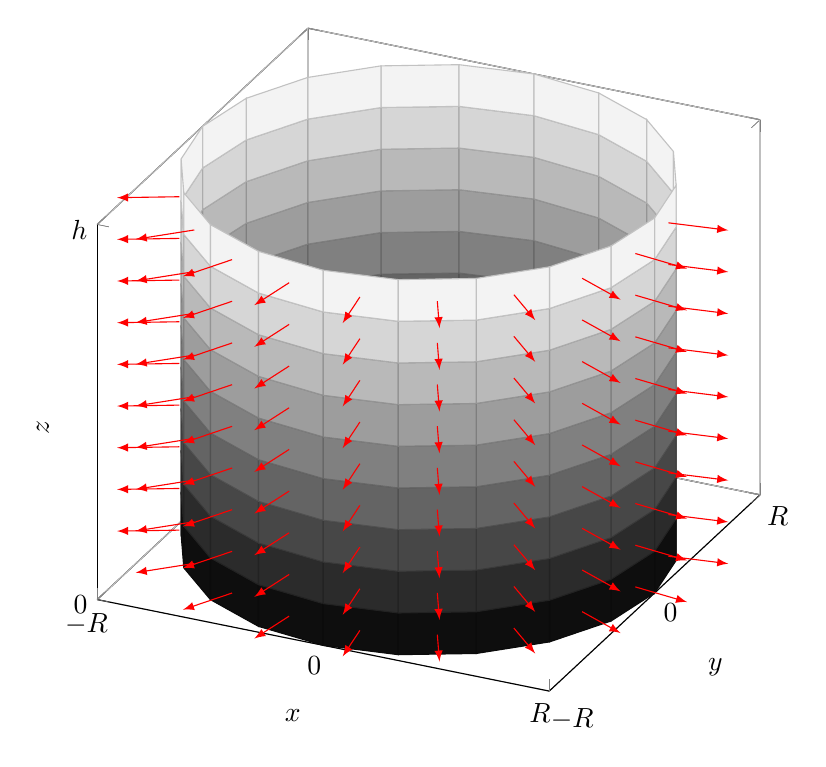
\begin{tikzpicture}
  \pgfmathsetmacro{\nphi}{20}
  \pgfmathsetmacro{\nz}{10}
  \begin{axis}[
    width=10cm,
    height=10cm,
    xlabel={$x$}, ylabel={$y$}, zlabel={$z$},
    xmin=-1,xmax=1,
    ymin=-1,ymax=1,
    zmin=0,zmax=1,
    % view={0}{90},
    grid,
    xtick={-1,0,1},
    xticklabels={$-R$,$0$,$R$},
    ytick={-1,0,1},
    yticklabels={$-R$,$0$,$R$},
    ztick={0,1},
    zticklabels={$0$,$h$},
    samples={\nphi+1}, samples y={\nz},
    z buffer=sort,
    clip=false,
    ]
    \addplot3[surf,colormap/blackwhite,domain={-pi/2}:{3*pi/2},domain y=0:1] ({cos(deg(x))},{sin(deg(x))},{y});
    \addplot3[red,
      quiver = {
        u = {x},
        v = {y},
        w = {0},
        scale arrows = 0.25,
        every arrow/.append style={-latex},
      },
      samples={\nphi/2}, samples y={\nz-1},
      domain={-pi + 2*pi/\nphi + pi/\nphi}:{2*pi/\nphi - pi/\nphi},
      domain y={1/18}:{1-1/18},
    ] ({cos(deg(x))},{sin(deg(x))},{y});
  \end{axis}
\end{tikzpicture}
\end{document}
